\documentclass[11pt]{article}

\usepackage[a4paper,margin=25mm]{geometry}
\usepackage{array}
\usepackage{booktabs}
\usepackage{enumitem}
\usepackage{graphicx}
\usepackage{hyperref}
\usepackage{tikz}
\usepackage{xcolor}
\usetikzlibrary{arrows.meta,positioning,calc}

\hypersetup{
  colorlinks=true,
  linkcolor=blue,
  urlcolor=blue,
  citecolor=blue
}

\setlist[itemize]{topsep=4pt,itemsep=2pt,parsep=0pt}
\setlist[enumerate]{topsep=4pt,itemsep=2pt,parsep=0pt}
\renewcommand{\arraystretch}{1.18}

\title{Logic Study Report for Textbook Enrichment\\
Sustainability and Resilience of Underground Infrastructure}
\author{Prepared for \textit{Underground Design and Construction}}
\date{Source presentation dated 30 July 2026; study report prepared 9 August 2026}

\begin{document}
\maketitle

\section*{Purpose of This Study Report}

This report reorganises the source presentation into a reader-oriented logic
study for the textbook \textit{Underground Design and Construction}. Rather
than following the order of presentation slides, it explains the material as a
connected learning sequence: why sustainability and resilience matter, how they
change underground design practice, and where the content should be added to
the textbook.

The source file is:

\begin{quote}
\texttt{Lecture Slides/2026.07.30 Sustainability and Resilience of Underground Infrastructure.pdf}
\end{quote}

The report is not a transcript. It is a structured interpretation for textbook
development, so the order below is governed by learning logic rather than by
presentation sequence.

\section*{Scope Note}

The source material should enrich the textbook primarily through digital lifecycle
management, carbon assessment, design optimisation, resilience assessment,
condition monitoring, and predictive maintenance. Slope-related material should
remain excluded from the main textbook in line with the earlier scope decision.
Where the source material includes a slope variable in a hydro-mechanical example,
the transferable content is the pressure-tunnel, leakage, hydro-mechanical
coupling, and carbon-assessment workflow; the slope-specific framing should not
be carried into the main text.

\section{Learning Logic for Readers}

The material should be taught as a lifecycle argument:

\begin{enumerate}
  \item Australia is in a period of major underground infrastructure delivery,
  including large transport tunnels, hydropower tunnels, stations, caverns, and
  service infrastructure.
  \item These projects face a high risk profile because ground movement,
  geological uncertainty, groundwater, induced seismicity, leakage, construction
  disturbance, and ageing can affect both construction safety and long-term
  service.
  \item Digital engineering is introduced as the organising framework for
  managing this complexity. The core data object is not just a geometric tunnel
  model, but a geo-integrated asset model linking ground, structure, process,
  performance, carbon, inspection, and decision records.
  \item Sustainability is then treated quantitatively through life-cycle carbon
  assessment, especially modules A1--A5, with particular attention to
  product emissions, transport, and construction energy from TBM excavation.
  \item Carbon reduction is positioned as a design optimisation problem, not
  only as a material substitution problem. Excavation disturbance, support
  distance, lining thickness, concrete strength, reinforcement ratio, and TBM
  performance all influence the final carbon baseline.
  \item Resilience is treated as time-dependent functionality under multiple
  hazards. The relevant question becomes how an underground asset loses
  function, how quickly it recovers, and how inspection and intervention can
  improve the life-cycle resilience index.
  \item Digital twins close the loop: sensing and inspection update the model;
  simulations forecast performance; decision modules select interventions; and
  the asset model is revised for the next cycle of management.
\end{enumerate}

This logic should be used to enrich the textbook as a single connected
workflow, rather than as separate isolated sections on BIM, carbon, and hazards.

\section{Schematic Logic of the Report}

Figure~\ref{fig:logic-schematic} summarises the recommended logic for readers.
The centre of the report is the geo-integrated digital asset model: it connects
ground uncertainty, infrastructure function, construction process, carbon
accounting, performance assessment, monitoring, and operation. Sustainability
and resilience are therefore not treated as separate add-ons; they are decision
criteria inside the same lifecycle model.

\begin{figure}[htbp]
\centering
\resizebox{\textwidth}{!}{%
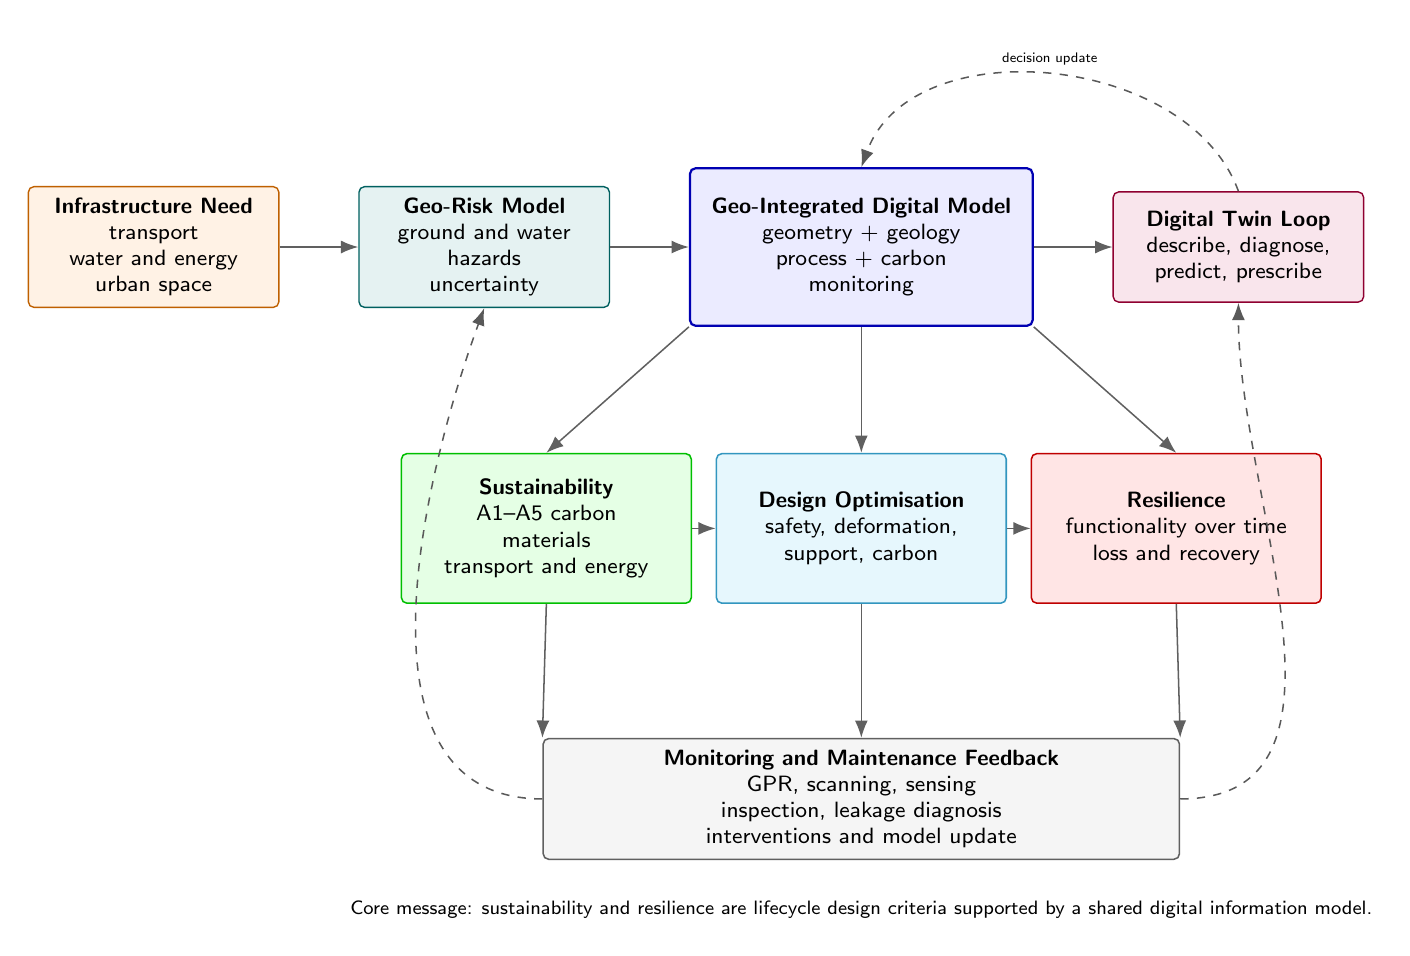
\begin{tikzpicture}[
  font=\sffamily\footnotesize,
  node distance=9mm and 10mm,
  box/.style={
    draw=#1!75!black,
    fill=#1!10,
    rounded corners=2pt,
    line width=0.5pt,
    align=center,
    text width=29mm,
    minimum height=14mm,
    inner sep=4pt
  },
  core/.style={
    draw=blue!70!black,
    fill=blue!8,
    rounded corners=2pt,
    line width=0.8pt,
    align=center,
    text width=40mm,
    minimum height=20mm,
    inner sep=5pt
  },
  module/.style={
    draw=#1!75!black,
    fill=#1!10,
    rounded corners=2pt,
    line width=0.55pt,
    align=center,
    text width=34mm,
    minimum height=19mm,
    inner sep=4pt
  },
  feedback/.style={
    draw=gray!75!black,
    fill=gray!8,
    rounded corners=2pt,
    line width=0.55pt,
    align=center,
    text width=78mm,
    minimum height=15mm,
    inner sep=4pt
  },
  arrow/.style={-{Latex[length=2.2mm]}, line width=0.55pt, draw=gray!75!black},
  feedbackarrow/.style={-{Latex[length=2.2mm]}, line width=0.55pt, draw=gray!70!black, dashed}
]

\node[box=orange] (need) {\textbf{Infrastructure Need}\\transport\\water and energy\\urban space};
\node[box=teal, right=of need] (risk) {\textbf{Geo-Risk Model}\\ground and water\\hazards\\uncertainty};
\node[core, right=of risk] (model) {\textbf{Geo-Integrated Digital Model}\\geometry + geology\\process + carbon\\monitoring};
\node[box=purple, right=of model] (twin) {\textbf{Digital Twin Loop}\\describe, diagnose,\\predict, prescribe};

\node[module=green, below=16mm of model, xshift=-40mm] (carbon) {\textbf{Sustainability}\\A1--A5 carbon\\materials\\transport and energy};
\node[module=cyan, below=16mm of model] (design) {\textbf{Design Optimisation}\\safety, deformation,\\support, carbon};
\node[module=red, below=16mm of model, xshift=40mm] (resilience) {\textbf{Resilience}\\functionality over time\\loss and recovery};

\node[feedback, below=17mm of design] (monitoring) {\textbf{Monitoring and Maintenance Feedback}\\GPR, scanning, sensing\\inspection, leakage diagnosis\\interventions and model update};

\draw[arrow] (need) -- (risk);
\draw[arrow] (risk) -- (model);
\draw[arrow] (model) -- (twin);
\draw[arrow] (model.south west) -- (carbon.north);
\draw[arrow] (model.south) -- (design.north);
\draw[arrow] (model.south east) -- (resilience.north);
\draw[arrow] (carbon.east) -- (design.west);
\draw[arrow] (design.east) -- (resilience.west);
\draw[arrow] (carbon.south) -- (monitoring.north west);
\draw[arrow] (design.south) -- (monitoring.north);
\draw[arrow] (resilience.south) -- (monitoring.north east);
\draw[feedbackarrow] (monitoring.west) to[out=180,in=250] (risk.south);
\draw[feedbackarrow] (monitoring.east) to[out=0,in=270] (twin.south);
\draw[feedbackarrow] (twin.north) to[out=110,in=70] node[above,align=center,font=\sffamily\tiny] {decision update} (model.north);

\node[align=center, font=\sffamily\scriptsize, below=4mm of monitoring] (captionnote)
{Core message: sustainability and resilience are lifecycle design criteria supported by a shared digital information model.};

\end{tikzpicture}%
}
\caption{Schematic logic for sustainable and resilient underground infrastructure.}
\label{fig:logic-schematic}
\end{figure}

\section{Reader-Oriented Logic Study}

\subsection{The Problem: Underground Infrastructure Is Becoming More Demanding}

Modern underground infrastructure is expanding rapidly in transport, water,
energy, hydropower, storage, and urban underground space. Australian projects
such as Melbourne Metro, North East Link, West Gate Tunnel, Suburban Rail Loop,
and Snowy 2.0 show the scale of this shift. These projects are valuable because
they support mobility, renewable energy, urban liveability, and infrastructure
capacity, but they also carry concentrated risks.

The reader should first understand that underground works are not only
construction projects. They are long-life public assets embedded in uncertain
ground. Their performance depends on excavation method, ground behaviour,
support and lining, groundwater, construction sequence, monitoring, maintenance,
and service disruption. This creates a natural need for lifecycle thinking.

\subsection{The Central Challenge: Risk, Carbon, and Service Life Are Coupled}

The source material links three problems that are often taught separately:

\begin{itemize}
  \item \textbf{Risk}: ground movement, sinkholes, settlement, leakage, induced
  seismicity, dynamic disturbance, and construction hazards can threaten safety
  and service.
  \item \textbf{Carbon}: tunnels contain large quantities of concrete, steel,
  grout, backfill, fit-out, excavation energy, spoil transport, and plant use.
  Carbon is therefore shaped by both design and construction process.
  \item \textbf{Resilience}: the asset must retain or recover functionality
  after deterioration, leakage, earthquake, blasting, operational transients, or
  other disruptive events.
\end{itemize}

The study logic is therefore: a sustainable underground asset is not simply a
low-carbon asset, and a resilient asset is not simply a strong asset. Good
underground design must balance safety, deformation, constructability, carbon,
maintainability, recovery, and uncertainty.

\subsection{The Information Backbone: Geo-Integrated Digital Modelling}

The next idea for readers is the need for a shared information backbone. A
tunnel model is not enough if it only contains geometry. A useful digital model
must integrate:

\begin{itemize}
  \item the infrastructure function and system interfaces;
  \item alignment, geometry, lining, support, shafts, stations, caverns, and
  fit-out;
  \item borehole information, geological interpretation, hydrogeological units,
  ground parameters, and uncertainty;
  \item construction method, sequence, support timing, TBM or excavation
  performance, and haulage assumptions;
  \item carbon quantities, carbon factors, energy factors, and system boundary;
  \item monitoring, inspection, condition, damage, leakage, and maintenance
  records.
\end{itemize}

This creates the foundation for geo-integrated BIM and digital twins. The
reader should see digital practice not as drawing management, but as the
structure that allows design, construction, carbon, risk, and operation to use
the same project information.

\subsection{The Sustainability Logic: Carbon Must Be Assessed by Life-Cycle Module}

The sustainability part of the material becomes understandable if organised by
life-cycle boundary. For tunnel construction, the key modules are:

\begin{itemize}
  \item \textbf{A1--A3 product stage}: concrete, steel, grout, backfill, lining
  components, fit-out, and other manufactured materials.
  \item \textbf{A4 transport}: material delivery and spoil haulage, controlled
  by transport distance, mode, fuel, vehicle type, and number of trips.
  \item \textbf{A5 construction}: construction energy, plant, TBM operation,
  excavation, spoil handling, dewatering, ventilation, cooling, and site energy.
  \item \textbf{B, C, and D stages}: maintenance, repair, replacement,
  operation, end-of-life processing, reuse, recovery, and recycling for broader
  whole-life assessment.
\end{itemize}

This should lead readers to the key message: carbon accounting must be based on
quantities, factors, and boundaries. Without these three elements, a reported
carbon number is difficult to compare or defend.

\subsection{The Design Logic: Carbon Is a Performance Variable}

The strongest textbook contribution is the idea that carbon should be part of
design optimisation. Carbon reduction does not only come from using lower-carbon
concrete. It can also come from reducing unnecessary excavation disturbance,
choosing an efficient support distance, optimising lining thickness and
reinforcement, improving TBM performance, reducing spoil transport, and
selecting construction methods that meet performance requirements without
overdesign.

This links sustainability to classical underground engineering. Factor of
safety, displacement, settlement, support pressure, construction risk, and
carbon become simultaneous design criteria. The reader should learn that a
low-carbon option is acceptable only if it remains safe, serviceable,
constructible, and robust under uncertainty.

\subsection{The Resilience Logic: Functionality Over Time}

Resilience should be taught through service functionality rather than only
through hazard intensity. The asset begins with a required level of function.
Ageing, creep, deterioration, leakage, earthquakes, blasting, operational
pressure transients, or other events can reduce that function. Inspection,
repair, strengthening, grouting, lining replacement, or other interventions can
restore function.

This leads to a practical resilience study sequence:

\begin{enumerate}
  \item define the service function;
  \item estimate baseline deterioration;
  \item apply hazard scenarios;
  \item calculate functionality loss and residual function;
  \item estimate delay and restoration time;
  \item evaluate recovery path;
  \item compute a resilience index;
  \item compare intervention options by function, time, carbon, cost, and risk.
\end{enumerate}

This is more useful for readers than treating earthquake, blasting, leakage, and
deterioration as separate topics with no shared lifecycle metric.

\subsection{The Digital Twin Logic: From Description to Prescription}

Digital twin content should be introduced after the reader understands the
asset, risk, carbon, and resilience logic. The digital twin then becomes the
method for closing the loop:

\begin{description}[leftmargin=34mm,style=nextline]
  \item[Descriptive] What is the asset? Geometry, geology, systems, materials,
  and records are organised into a structured model.
  \item[Reflective] What is happening now? Monitoring, machine data, inspection,
  sensing, and condition observations validate and update the model.
  \item[Predictive] What will happen next? Physical models, statistical models,
  machine learning, and surrogate models forecast settlement, convergence,
  leakage, deterioration, damage, energy, carbon, and functionality.
  \item[Prescriptive] What should be done? Intervention options are compared
  using risk, recovery, cost, time, carbon, and service outcomes.
\end{description}

This gives the reader a clear progression from digital records to digital
decision-making.

\subsection{The Inspection and Maintenance Logic: Monitoring Closes the Loop}

The final concept is that operation and maintenance complete the engineering
cycle. Technologies such as geometry scanning, GPR, LiDAR, photogrammetry,
computer vision, microseismic sensing, leakage observations, and virtual sensing
are valuable because they update the asset model. The purpose is not merely to
collect more data, but to support condition diagnosis, predictive maintenance,
early warning, and lower-carbon intervention.

In this logic, a good inspection programme has three outputs:

\begin{itemize}
  \item an updated diagnosis of current condition;
  \item a prediction of future performance and risk;
  \item a decision on whether, when, and how to intervene.
\end{itemize}

This makes monitoring part of design continuity rather than an isolated
operational task.

\section{Recommended Textbook Workflow}

The reader-oriented logic can be converted into the following textbook workflow.

\subsection{Workflow 1: From Infrastructure Need to Geo-Risk Model}

\begin{enumerate}
  \item Define the infrastructure function: transport, energy, water, storage,
  underground space, or lifeline service.
  \item Identify constraints: alignment, depth, interfaces with existing assets,
  construction access, settlement tolerance, groundwater, programme, and carbon
  targets.
  \item Build the geological and hydrogeological interpretation from boreholes,
  geophysics, mapping, laboratory tests, and historical project data.
  \item Convert the interpretation into explicit geo-uncertainty classes:
  material uncertainty, boundary uncertainty, groundwater uncertainty, structural
  uncertainty, and construction-process uncertainty.
  \item Link uncertainty to hazards: ground movement, instability, leakage,
  construction disturbance, machine performance risk, durability loss, dynamic
  disturbance, and recovery demand.
  \item Define the information model required to manage these risks across
  planning, design, construction, and operation.
\end{enumerate}

\subsection{Workflow 2: Geo-Integrated BIM and Analysis Loop}

\begin{enumerate}
  \item Create the base asset model: alignment, stations, caverns, shafts,
  tunnel geometry, lining, support, fit-out, and interfaces.
  \item Add the ground model: strata, inferred boundaries, hydrogeological
  units, structural features, design parameters, uncertainty ranges, and
  chainage-based classification.
  \item Assign semantic attributes: material properties, construction sequence,
  support type, monitoring points, carbon factors, quantities, and inspection
  records.
  \item Select an appropriate level of detail for the decision being made. Early
  planning may use system-level quantities; detailed design and operation need
  component- and material-level information.
  \item Instantiate analysis models from the BIM and ground model, including
  settlement, support interaction, lining response, excavation sequence, and
  construction energy where relevant.
  \item Run forward analysis to predict performance, then use backward feedback
  from observations and validation data to update parameters, refine design, or
  change construction control.
  \item Keep the loop active through construction and operation rather than
  treating BIM as a static drawing container.
\end{enumerate}

\subsection{Workflow 3: Life-Cycle Carbon Assessment for Tunnels}

\begin{enumerate}
  \item Define the system boundary using EN 15978 / EN 17472 terminology. The
  key construction-stage boundary highlights A1--A3 product emissions, A4 transport, and A5 construction,
  with later-life modules B, C, and D available for whole-life studies.
  \item Extract quantities from the digital asset model: lining concrete,
  reinforcement, backfill, grout, fit-out, rail or road deck, spoil, and
  equipment-related quantities.
  \item Assign carbon factors from databases, environmental product
  declarations, project data, or user-defined factors. Concrete strength,
  supplementary cementitious materials, steel type, and geographical context
  should be recorded explicitly.
  \item Calculate product emissions for A1--A3 from quantity and carbon factor.
  For lining assessment, key drivers include internal diameter, thickness,
  concrete grade, reinforcement ratio, and reinforcement type.
  \item Calculate A4 transport emissions from haulage distance, mode, mass or
  volume, trip number, and vehicle or energy factor.
  \item Calculate A5 construction emissions. For TBM tunnelling, energy is
  project-specific because torque, thrust, rate of
  penetration, rotation speed, diameter, depth, ground type, and in-situ stress
  affect excavation energy.
  \item Establish a baseline and test reduction scenarios, including lower
  carbon concrete, supplementary cementitious materials, reinforcement
  optimisation, reduced lining thickness where justified, spoil haulage
  reduction, recycled or remanufactured components, and TBM performance
  optimisation.
  \item Report both the total carbon and the drivers, because the best reduction
  lever changes between planning, reference design, detailed design, and
  construction.
\end{enumerate}

\subsection{Workflow 4: Geo-Structural Carbon Optimisation}

The key textbook message is that carbon reduction is coupled to geotechnical
performance. A defensible optimisation workflow is:

\begin{enumerate}
  \item Define design variables: lining thickness, concrete strength, support
  distance from the face, reinforcement ratio, support type, excavation method,
  and construction control variables.
  \item Define geotechnical inputs and uncertainty ranges: in-situ stress,
  ground class, stiffness, strength, groundwater, and excavation disturbance.
  \item Define performance constraints: factor of safety, support pressure,
  deformation, settlement, serviceability, constructability, and durability.
  \item Define the carbon objective using module-based emissions, at minimum
  A1--A5 for design decisions during construction.
  \item Evaluate feasible design alternatives using analytical methods,
  convergence-confinement calculations, numerical modelling, or surrogate
  models, depending on project stage.
  \item Use multi-objective optimisation to identify Pareto solutions rather
  than a single minimum-carbon option. The preferred option should satisfy
  safety and deformation constraints while avoiding unnecessary support demand.
  \item Interpret results physically: allowing controlled ground deformation,
  optimising support distance, or improving excavation control may reduce
  structural demand and carbon, provided serviceability and construction risks
  remain acceptable.
\end{enumerate}

\subsection{Workflow 5: Digital Twin for Sustainable and Resilient Management}

The digital twin logic can be organised into four maturity levels:

\begin{description}[leftmargin=34mm,style=nextline]
  \item[Descriptive twin] Defines what the asset is. It integrates geometry,
  geology, structure, systems, materials, historical data, and semantic
  attributes into an informatised asset model.
  \item[Reflective twin] Explains what is happening and why. It ingests sensing,
  inspection, machine data, structural monitoring, and condition records to
  validate the model and diagnose the current state.
  \item[Predictive twin] Forecasts what will happen. It combines physical,
  statistical, machine-learning, and multi-physics models to estimate settlement,
  convergence, leakage, damage, deterioration, energy, carbon, and service
  functionality.
  \item[Prescriptive twin] Recommends what should be done. It compares
  intervention schemes, restoration options, risk criticality, carbon impact,
  cost, delay, and expected recovery of functionality.
\end{description}

This four-level structure should become a major organising device for the
digital underground and asset-management chapters.

\subsection{Workflow 6: Resilience Assessment and Restoration}

\begin{enumerate}
  \item Define the service function of the asset, expressed as a functionality
  curve over time.
  \item Establish baseline life-cycle performance under ageing, creep,
  deterioration, leakage, or other long-term mechanisms.
  \item Add discrete hazards such as earthquake, blasting, operational pressure
  transients, leakage-induced disturbance, impact, or construction events.
  \item Estimate vulnerability and robustness by quantifying functionality loss
  immediately after the event.
  \item Estimate delay time and restoration time for each intervention option.
  \item Calculate a resilience index from the recovered functionality over the
  recovery window, while documenting residual functionality, recovery shape, and
  uncertainty.
  \item Compare restoration schemes by functionality recovery, time, cost,
  constructability, risk reduction, and carbon impact.
  \item Feed inspection and post-intervention data back into the digital twin.
\end{enumerate}

\section{Chapter Integration Map}

\subsection*{\texttt{ch01-infrastructure-and-challenges.tex}}

Add the Australian underground infrastructure boom, infrastructure risk
dashboard, ground movement examples, Snowy 2.0 and Melbourne Metro as
motivating cases, and the combined drivers of digitalisation, sustainability,
and resilience. This strengthens the opening rationale for modern underground
engineering as a high-risk, high-carbon, high-value infrastructure discipline.

\subsection*{\texttt{ch05-site-investigation.tex} and \texttt{engineering-geology.tex}}

Add geo-uncertainty identification, borehole-based geological interpretation,
regional hydrogeological and geological modelling, and uncertainty classes
needed for digital modelling. This connects site investigation to downstream
digital and analytical workflows, instead of treating investigation as a
stand-alone data collection exercise.

\subsection*{\texttt{ch08-numerical-modelling.tex} and \texttt{advanced-numerical.tex}}

Add model instantiation from BIM, forward and backward loops, parametric
analysis, validation, surrogate modelling, and multi-fidelity coupling. This
shows students how numerical models are created, updated, and used inside a
project information workflow.

\subsection*{\texttt{ch09-integrated-design.tex}}

Add geo-structural-carbon optimisation, Pareto trade-offs, factor of safety
versus deformation versus carbon, and uncertainty-informed decision making.
This turns integrated design into a practical optimisation framework with
explicit sustainability criteria.

\subsection*{\texttt{ch10-construction-methods.tex} and \texttt{tbm-engineering.tex}}

Add TBM performance links to A5 carbon: torque, thrust, rate of penetration,
rotation speed, diameter, ground-machine interaction, spoil removal, and
construction energy. This adds a quantitative sustainability dimension to
construction-method selection and TBM performance assessment.

\subsection*{\texttt{segmental-linings.tex}, \texttt{support-interaction.tex}, and \texttt{final-linings.tex}}

Add lining carbon baseline, internal diameter/thickness ratio, concrete
strength, SCM substitution, reinforcement ratio, support distance, and
controlled deformation as carbon-sensitive design variables. This shows that
support and lining design affects carbon through geometry, materials, timing,
and mobilisation of ground-support interaction.

\subsection*{\texttt{sustainability.tex}}

Add life-cycle module boundary, A1--A5 workflow, carbon-factor databases, TunCO2
style carbon accounting, baseline and reduction-potential logic, and staged
decision leverage from planning to detailed design. This is the main direct
enrichment target.

\subsection*{\texttt{digital-underground.tex}}

Add object-oriented BIM, IFC/semantic enrichment, LoD, geological model
integration, and the descriptive-reflective-predictive-prescriptive twin
structure. This makes digital engineering more than visualisation: it becomes
the operating system for risk, carbon, construction, and asset decisions.

\subsection*{\texttt{monitoring.tex} and \texttt{asset-management.tex}}

Add GPR inspection, geometry scanning, computer vision, microseismic sensing,
condition assessment, predictive datasets, virtual sensing, leakage detection,
and model updating. This provides the operational feedback loop needed for
lifecycle resilience and predictive maintenance.

\subsection*{\texttt{risk-and-delivery.tex}, \texttt{construction-hazards.tex}, and \texttt{seismic-design.tex}}

Add multi-hazard resilience workflow, functionality loss, robustness, delay,
restoration, resilience index, and intervention selection. This moves hazard
treatment from event-by-event design checks toward lifecycle functionality and
recovery.

\section{Proposed New Textbook Logic}

The book currently contains separate chapters on digital practice,
sustainability, risk, monitoring, and asset management. This study report
recommends cross-linking them through a shared lifecycle workflow:

\begin{center}
\begin{tabular}{>{\raggedright\arraybackslash}p{0.19\textwidth}
                >{\raggedright\arraybackslash}p{0.70\textwidth}}
\toprule
\textbf{Stage} & \textbf{Core logic} \\
\midrule
Need and context &
Why underground infrastructure is selected; what service it provides; what
carbon, risk, resilience, and social constraints govern the project. \\
Ground and asset model &
How the ground, water, structure, construction sequence, and asset components
are represented in a digital model. \\
Design and analysis &
How settlement, support interaction, lining response, machine performance,
and construction hazards are analysed. \\
Carbon and optimisation &
How the design is tested against A1--A5 carbon, safety, deformation,
constructability, and uncertainty. \\
Construction feedback &
How machine data, monitoring, observations, and as-built records validate or
revise the model. \\
Operation and resilience &
How deterioration, leakage, dynamic events, inspection, restoration, and
functionality recovery are modelled over service life. \\
Digital twin closure &
How each observation and intervention updates the model for the next decision.
\\
\bottomrule
\end{tabular}
\end{center}

\section{Chapter-Ready Section Suggestions}

\subsection*{For the Sustainability Chapter}

\begin{itemize}
  \item Add a section titled \textit{Model-based carbon assessment for tunnels}.
  The section should explain that tunnel carbon assessment depends on a digital
  quantity model, a carbon-factor library, a system boundary, and a construction
  process model.
  \item Expand the existing carbon assessment section with EN 15978 /
  EN 17472 module language: A1--A3 product, A4 transport, A5 construction, B
  use and maintenance, C end of life, and D beyond-system benefits.
  \item Add a TBM-specific subsection for A5 construction emissions. Explain
  that excavation energy should be estimated from ground-machine interaction,
  not assigned as a generic percentage.
  \item Add a subsection on baseline and reduction potential. The baseline
  should be defined by diameter, lining thickness, concrete grade, reinforcement
  ratio, transport assumptions, and construction energy.
  \item Add a design box on carbon levers: SCM substitution, concrete strength
  selection, reinforcement optimisation, support distance, lining thickness,
  excavation disturbance, spoil transport, and TBM performance.
\end{itemize}

\subsection*{For the Digital Underground Chapter}

\begin{itemize}
  \item Add a workflow figure or algorithm for geo-integrated BIM:
  asset model + ground model + semantic attributes + analysis model +
  validation + update.
  \item Introduce the four digital twin stages: descriptive, reflective,
  predictive, and prescriptive.
  \item Emphasise levels of detail as decision-dependent: LoD for planning,
  reference design, detailed design, construction control, and operation should
  not be the same.
  \item Add a short discussion of interoperability and semantic enrichment:
  geometry alone is insufficient unless material properties, ground classes,
  construction sequence, monitoring records, and carbon factors are attached.
\end{itemize}

\subsection*{For Integrated Design and Numerical Modelling}

\begin{itemize}
  \item Add carbon as an explicit objective beside factor of safety,
  displacement, settlement, cost, and constructability.
  \item Use the optimisation logic to introduce Pareto design decisions:
  there may be no single best design, only a defensible trade-off between
  performance and carbon.
  \item Explain that controlled deformation can sometimes reduce support demand
  and carbon, but only within serviceability, construction, and risk limits.
  \item Include genetic algorithm or surrogate-model optimisation as an
  advanced method after simpler parametric comparisons.
\end{itemize}

\subsection*{For Resilience, Monitoring, and Asset Management}

\begin{itemize}
  \item Add a resilience-index section based on functionality over time,
  vulnerability, robustness, delay, restoration, and recovered functionality.
  \item Connect inspection methods to model updating: GPR, LiDAR, photogrammetry,
  computer vision, microseismic sensing, and leakage observations should be
  framed as data streams into a digital twin.
  \item Add predictive maintenance logic: surface observation plus internal
  inspection plus multiphysics modelling can move asset management from
  reactive repair to forecast-based intervention.
  \item Treat restoration options as engineering design decisions with carbon
  and service consequences, not merely maintenance activities.
\end{itemize}

\section{Important Technical Concepts to Carry Forward}

\subsection*{Carbon Boundary and Formula Logic}

The source material repeatedly uses the idea that total construction-stage carbon for a
tunnel can be assembled from material, transport, and construction-process
terms:

\[
GWP_A = \sum_i V_i \left(GWP_{i,A1-A3} + GWP_{i,A4}\right) + GWP_{A5}
\]

For TBM excavation, the construction-stage term can be tied to energy demand:

\[
GWP_{A5} = E_{\mathrm{TBM}} \left(EF_2 + EF_3\right)
\]

In the textbook, these equations should be introduced as accounting logic
rather than as universal closed-form design equations. The important point is
that carbon calculations must be traceable to quantities, system boundaries,
carbon factors, energy factors, and modelling assumptions.

\subsection*{Design Variable Hierarchy}

The study logic indicates that carbon sensitivity can arise from:

\begin{itemize}
  \item alignment, depth, diameter, and geometric scale;
  \item lining thickness, concrete grade, SCM content, and reinforcement ratio;
  \item support distance and mobilisation of ground-support interaction;
  \item excavation method and disturbance;
  \item TBM performance, including thrust, torque, rate of penetration, and
  construction energy;
  \item spoil removal distance and transport mode;
  \item restoration strategy and timing during operation.
\end{itemize}

This hierarchy should be used to avoid over-emphasising material substitution.
The larger textbook message is that early design and construction-control
decisions often dominate the achievable carbon reduction.

\subsection*{Resilience Metrics}

The resilience discussion should be framed around:

\begin{itemize}
  \item initial service functionality;
  \item hazard occurrence time;
  \item immediate functionality loss;
  \item residual functionality;
  \item delay before restoration;
  \item recovery trajectory;
  \item final restored functionality;
  \item area under the functionality-time curve;
  \item uncertainty in hazard intensity, damage, detection, and recovery.
\end{itemize}

This provides a practical bridge between hazard analysis and asset management.

\section{Suggested Figures and Tables for Later Book Enrichment}

\begin{enumerate}
  \item A lifecycle workflow diagram from planning to operation, showing
  ground model, asset model, carbon model, performance model, monitoring data,
  and decision feedback.
  \item A table of EN 15978 / EN 17472 modules with tunnel-specific examples:
  concrete, steel, grout, spoil transport, TBM electricity, ventilation,
  maintenance, demolition, reuse, and recycling.
  \item A Pareto trade-off figure showing carbon versus factor of safety and
  deformation. This can be a schematic in the textbook if original data are not
  reused.
  \item A digital twin maturity figure with descriptive, reflective, predictive,
  and prescriptive layers.
  \item A resilience functionality-time curve showing vulnerability,
  robustness, delay, recovery, and restoration.
  \item A monitoring-to-model-update workflow for GPR, scanning, computer
  vision, microseismic sensing, and leakage detection.
\end{enumerate}

\section{Editorial Cautions}

\begin{itemize}
  \item Keep the textbook language at teaching level. Some source examples contain
  research-frontier material; it should be introduced through concepts,
  workflows, examples, and optional advanced boxes rather than dense
  publication-style detail.
  \item Avoid making the sustainability chapter a list of carbon factors. The
  most valuable contribution is the connection between design decisions,
  construction method, ground uncertainty, and carbon.
  \item Avoid making the digital chapter a software chapter. The important
  teaching concept is information flow and decision traceability.
  \item Do not reintroduce slope-related content into the main book. Where a
  source example contains slope variables, retain only the underground asset
  logic if it is transferable.
  \item Separate established design practice from emerging research methods.
  Digital twins, synthetic GPR datasets, and prescriptive maintenance should be
  presented as forward-looking methods unless supported by mature project case
  evidence.
\end{itemize}

\section{Immediate Enrichment Priority}

For the next textbook editing pass, the highest-value additions are:

\begin{enumerate}
  \item Enrich \texttt{sustainability.tex} with A1--A5 model-based tunnel carbon
  assessment and TBM-specific A5 construction energy.
  \item Enrich \texttt{digital-underground.tex} with the geo-integrated BIM loop
  and the four-level digital twin framework.
  \item Enrich \texttt{ch09-integrated-design.tex} with carbon-performance
  Pareto optimisation and design-variable sensitivity.
  \item Enrich \texttt{asset-management.tex} and \texttt{monitoring.tex} with
  inspection, predictive maintenance, resilience index, and restoration
  decision logic.
  \item Add cross-references from \texttt{tbm-engineering.tex} to sustainability
  where TBM performance, spoil removal, and electricity use affect A5 carbon.
\end{enumerate}

\end{document}
